\documentclass[../main.tex]{subfiles}
\graphicspath{{\subfix{../}}}
\begin{document}


%The Information Modeling Framework (IMF) is a method, a framework, and a language that allows creating a formal description of a Facility Asset, using common industry reference data libraries containing definitions of elements that are frequently re-used. The resulting Information Model of the Facility Asset contains information in a format which is readable to humans as well as to computers.

\chapter{Scope}
\label{ch:Chapter 1}

This document contains a specification of the Information Modelling Framework (IMF), including 
 fundamental concepts and guidelines for use, as well as
its intended working relations to external resources and applications. Referring to \autoref{fig:Figure 2} the external resources and applications are: 
 \begin{itemize}
     \item[\ding{182}]  Engineering tools and registers that hold attributes and objects that are part of the information model describing the facility asset. 
     \item[\ding{183}]  Modelling tools for creating, modifying, and sharing IMF models.
\item[\ding{184}]  Reference data libraries that contain resources used when building IMF models. 
\item[\ding{185}]  Semantic verification mechanisms and tools that offer computer-based validation, integrity checking, and verification of the
IMF model.
\end{itemize}

\begin{figure}[h]
  \centering
  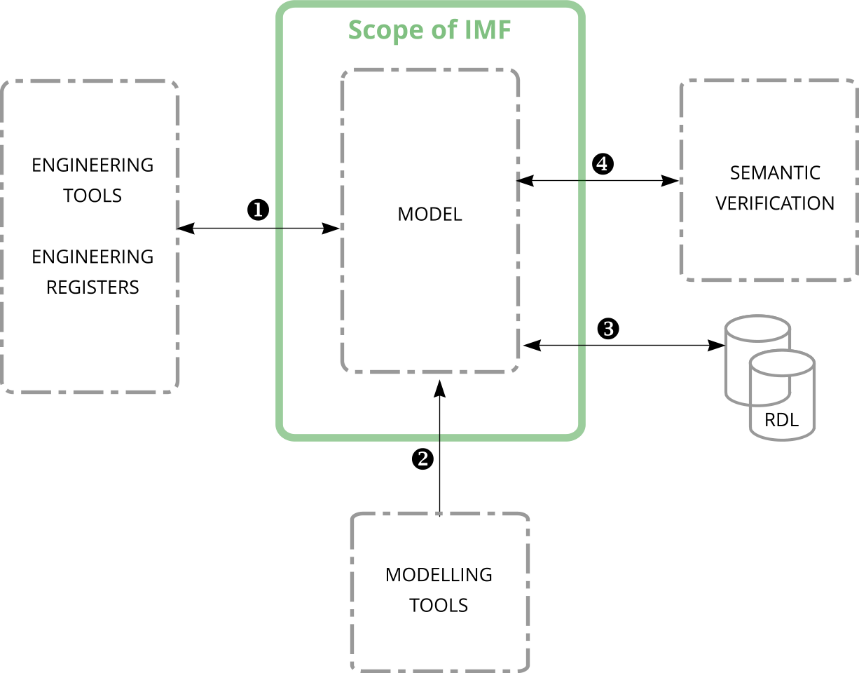
\includegraphics[width=.7\textwidth]{img/IMFmanual-img002.png}
  \caption{Framing and scoping of the IMF.}
  \label{fig:Figure 2}
\end{figure}


%This Manual specifies the framework and language IMF shall possess if it is to serve such purposes in support of the goals of automated exchange, retrieval, integration and analysis of Facility Asset data by computer systems.

%\newpage
The following are within the scope of this manual:
\begin{itemize}
    \item A definition of the IMF language, including vocabulary and rules.
    \item A description of interfaces to external systems being part of the ecosystem.
    \item A definition of a modelling methodology.
    \item A definition of a methodology for creating or modifying modelling building blocks.
    \item Guidelines that enable subject matter experts (SMEs) to be users of the framework, supporting and improving existing discipline design workflows.
    \item Identification of modelling tools for creating, modifying, and sharing IMF models. 
    \item Explanation of use of reference data libraries that contain the resources from which IMF models are built. 
    \item Semantic verification mechanisms and tools that offer computer-based validation and verification of the IMF model.
    %\item Processes and artefacts that are scalable across disciplines, work processes, and the value chain, supporting any level of complexity and level of detail, and depending on the need and where in the process the SMEs are.
    \item Open protocols for exchange of facility asset information and formats that enable automated verification and augmented engineering extensions.
    \item Examples of shared libraries and use of existing standards.
    \item Examples of engineering tools and engineering registers that may hold attributes and objects and describe the facility asset.
\end{itemize}

%The following are out of scope of this Manual:

%Normative references

%Terms and definitions

%The following is included in the scope:

%\begin{itemize}
%  \item Definition of the IMF language, including vocabulary and rules.
%  \item Description of interfaces to external systems being part of the ecosystem.
%  \item Specification of modelling methodology.
%  \item Specification of methodology for creating or modifying modelling building blocks.
%\end{itemize}

%\section{Industry Value of the Work}
This document and the development of IMF is intended to serve as a reference for:

\begin{itemize}
  \item Understanding how to implement a new way of working using information models.
  \item The basis for a DNV recommended practice on the subject of creating and using of industrial facility assets information models.
  \item Implementing tools and applications for information modelling.
  \item Alignment of industry reference data libraries.
  \item Implementation of cross-industry interoperability based on IEC/ISO 81346-1~\cite{81346-1} (structuring principles) and
        ISO 15926-14~\cite{15926-14} (reference data and verification).
  \item Computer-based exchange, automation, and verification of information models.
%  \item Contractual requirements for delivery of facility asset information models. See \autoref{ch:Appendix B}.
\end{itemize}

\end{document}